%!TEX root = ../../../ECP-ST-CAR.tex 

\subsubsection{\stid{5.10} ExaWorks} \label{subsubsect:exaworks}

% ECP ST Project Overviews: A significant portion of this report includes 2-page synopses of each
% ECP ST project (Section 4), including a project overview, key challenges, solution strategy, recent progress and next steps

\paragraph{Overview} 
Exascale computers will offer transformative capabilities to combine
data-driven and learning-based approaches with traditional simulation
applications to accelerate scientific discovery and insight. These software
combinations and integrations, however, are difficult to achieve due to
challenges coordinating and deploying heterogeneous software components
on diverse and massive platforms. The ExaWorks project is addressing 
these challenges by co-designing an open Software Development Kit (SDK) 
consisting of workflow management systems (WMSs) that can be
composed and interoperate through common interfaces. 
The project is working to bootstrap the SDK with an initial
set of tools, design common interfaces, make tools
easier to apply to complex science challenges, 
and apply the SDK to ECP applications.
The project is community centered, 
working with stakeholders, including
users, developers, and facility representatives, to 
sustainably address workflows requirements at
exascale.




\paragraph{Key Challenges}
Emerging exascale workflows pose significant challenges to the creation of
portable, repeatable, scalable, and performant workflows. These challenges are both
technical and non-technical. On the technical side, WMSs are 
incapable of supporting heterogeneous co-scheduled and
high-throughput workflows, and enabling communication between fine-grained
tasks in dynamic workflows. On the non-technical side, the myriad WMSs
that exist, absence of reusable WMS components, and lack of user
guidance when selecting a WMS has led to a disjoint workflows community
that tends toward building ad hoc or bespoke solutions rather than adopting
and extending existing solutions. Important challenges include: 
\begin{enumerate}
    \item Workflows community: the workflows, applications, and facility communities are disjoint. 
    Efforts are needed to bring these groups together to define, develop, and integrate common workflow components. % and interfaces. 
    %and to work together to develop, integrate, and support these components.
    \item Scheduling: exascale workflows must manage the efficient execution of diverse
    tasks (e.g., in runtime, resource requirements, single/multi-node) with complex interdependencies on heterogeneous resources. 
    \item Scale and performance: emerging workflows feature huge ensembles of short-running jobs, 
    which can create millions or even billions of tasks that need to be rapidly scheduled and executed.
    \item Coordination and communication: workflows depend on coordination between the workflow and 
    the tasks within it, a need that requires efficient exchange of data following various communication patterns.
    %\item Fault tolerance: the enormous number of computing elements and workflow tasks increases 
    %the likelihood of encountering faults within a workflow at the system level and from the millions of concurrent tasks. 
    \item Portability: WMSs are tested on a handful of systems and the frequency by which
    system hardware and software change makes it impossible to guarantee that a workflow will work on a system in the future.
\end{enumerate}

\begin{wrapfigure}{r}{0.4\textwidth}
\begin{center}
    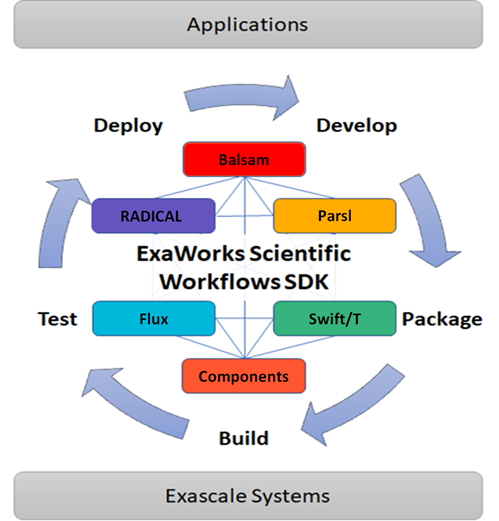
\includegraphics[width=0.37\textwidth]{projects/2.3.5-Ecosystem/2.3.5.10-ExaWorks/exaworks-circle.png}
  \end{center}
  \vspace{-0.25in}
  \caption{ExaWorks Toolkit\label{fig:arch}}
\end{wrapfigure} 

\paragraph{Solution Strategy}
The ExaWorks project lays the foundation for an inherently
\textit{new approach} to workflows: establishing an SDK (see
Figure~\ref{fig:arch}) by assembling components from existing WMSs
and defining new component interfaces. 
The ExaWorks SDK provides a robust, well-tested, well-documented,
and scalable set of tools and components that can be combined to enable diverse teams to
produce scalable and portable workflows for a wide range of exascale
applications. Importantly, the project is not creating a new workflow system
nor does it aim to replace the many workflow solutions already deployed
and used by scientists, but rather it will provide well-engineered and
scalable SDK which can be leveraged by new and existing workflows.


%\begin{wrapfigure}[0]{r}{0.5\textwidth}


The goals of the first year of the project are to instantiate the ExaWorks SDK, seed the SDK with
robust workflow component technologies, explore pairwise integrations between components, and define
common component interfaces.  The project also aims to impact ECP applications and
bring together the workflows community, including developers, ECP applications, and DOE compute facility representatives
to collectively address workflows challenges.
%.  Specifically, it will:
% \begin{enumerate}
%     \item Engage the facilities to survey the state of workflow tools and capabilities and ways in which ExaWorks can enhance their capabilities;
%     \item Establish an advisory board composed of representatives of DOE compute facilities, ECP applications, and workflow tools, to guide and advise ExaWorks;
%     \item Survey ECP applications teams to identify the tools currently being used and to identify common challenges and needs;
%     \item Assemble a functional design working group to develop a community-centered draft function design; and
%     \item Collaborate with ECP applications to develop a proof-of-concept integration using a shared functional component as defined by the draft design, in an ECP application.
% \end{enumerate}

\paragraph{Recent Progress}
% In this period of the project we have
% assembled our advisory committee, 
% started a functional design working group, and distributed a workflows
% survey to the ECP community. The results of this survey are helping
% to prioritize in-person interviews as well as informing the 
% functional design process and helping to identify initial ExaWorks components. 
% Our team have started prototyping efforts to explore 
% component-based approaches in existing workflow systems. Specifically, 
% we have developed prototype Balsam and RADICAL-Pilot executors for Parsl
% which enable Parsl workflows to leverage the resource management 
% capabilities of these external systems.



In this period of the project we have focused on addressing our goals outlined above. 
%instantiating the SDK, defining and developing
%the first component interface, working with ECP applicaiton teams, and engaging
%the workflows community. 
We briefly describe efforts in each area. 

We released the first version of the ExaWorks SDK. We first defined
community policies~\cite{sdk-policies} (modeled on E4S) and
developed a GitHub Actions-based continuous integration model and 
a Spack-based packaging approach. 
Our packaging solutions allow for portable and reproducible deployment and 
testing techniques, which vary considerably among WMSs.
We have bootstrapped the SDK with five workflow technologies 
that are widely used in ECP applications. We followed a community-based
approach in which all artifacts are tracked using an open process on GitHub. 
%We have defined a Fork+Pull model-based GitHub development workflow and and 
%GitHub Actions-based continuous integration testing and deployment for SDK components.

Based on feedback from the ECP workflows community, we identified our 
first component interface for the SDK: PSI/J, a portability layer across different HPC workload managers. 
%allowing workflow developers and users to create portable workflows with a standard API. 
%Our survey highlighted the challenge of porting workflows as one of the most critical needs for workflow developers and users alike. 
As a community, we defined a language-agnostic specification~\cite{jpsi-spec}
and after iteration released a first version of the specification. 
We have also released a 0.1 version of Python implementation~\cite{jpsi-python}. 
The Python library contains the set of
core classes defined by the specification, as well as abstract base classes (ABCs) for components 
that implement functionality specific to different clusters and batch systems.
The implementation currently supports Slurm, LSF, Cobalt, RADICAL-Pilot, and Flux connectors. 

We have continued to work closely with several ECP applications, including 
ExaLearn, CANDLE, and ExaAM.
 %ExaLearn and CANDLE through ongoing
%collaborations, and have strengthened collaborations with the ExaAM team. 
As the ExaAM workflow is in its early stages, we are using this engagement
as a way of defining processes for engaging with new ECP teams in the future.  
The ExaAM workflow is composed of several application codes, each capturing a
different scale or physics of the problem.  Each stage feeds
information to the next stage, and iteration can occur across stages.  Some
stages leverage CPU's and others GPU's. Several stages are themselves small
workflows typically leveraging the \textit{ensemble} motif. Thus, the ExaAM
workflow requires integration of multiple physics applications and when
executed at full scale will require complex orchestration of many
sub-workflows.  
%The ExaAM collaboration provides a strong vehicle for co-design and informing the 
%ExaWorks SDK. 
Initial integration of ExaWorks SDK technologies has shown that
improvements in throughput are possible with minor changes to existing scripts.
%The ExaAM and ExaWorks teams have identified additional stages in the workflow
%that could benefit by incrementally integrating ExaWorks SDK capabilities to
%improve portability and performance.  In order to facilitate this engagement,
%the ExaAM team has produced an example workflow capability of being executed
%upon ECP CI infrastructure and that will be used to demonstrate integration of additional
%ExaWorks SDK components.

In collaboration with the NSF-funded WorkflowsRI project, we are hosting a
series of workflows community summits that aim to bring the workflows
community together~\cite{dasilva2021community}. The first
summit~\cite{summit-1} brought together 48 international participants
representing many WMSs, with the goal to identify crucial challenges in the
workflows community. The summit considered six broad themes: FAIR workflows,
training and education, AI workflows, exascale challenges, APIs and
interoperability, and developing workflow community. The second
summit~\cite{summit-2} focused on technical approaches for realizing many of
the challenges identified in the first summit. It included 75 workflows
developers %from around the world
and focused on three core topics: defining common workflow patterns and
benchmarks, identifying paths toward interoperability of workflow systems, and
improving workflow systems' interface with legacy and emerging HPC software
and hardware. The third workshop (scheduled for early November 2021) will
explore workflows challenges and opportunities from the perspective of
computing centers and facilities.  It will bring together a small group of
facilities representatives with the aim to understand how workflows are
currently being used at each facility, how facilities would like to interact
with workflow developers and users, how workflows fit with facility roadmaps,
and what opportunities there are for tighter integration between facilities
and workflows. We also host an open monthly community meeting that is attended
by representatives across DOE laboratories. A snapshot of progress and plans
of ExaWorks was accepted for the SC21 workshop on workflows
(WORKS21)~\cite{alsaadi2021exaworks}.


\paragraph{Next Steps}
% The remainder of this initial effort focuses on four important areas. 
% First, continuing to grow the ExaWorks community by engaging with ECP 
% applications, facilities, and WMS teams. 
% Second, working with these partners and stakeholders to produce a draft
% functional design document that outlines ExaWorks components
% and potential interfaces to these components. 
% Third, we will produce a report, derived from interviews from 
% the broad ECP community that outlines ECP workflows needs, challenges, 
% and potential solutions. 
% Finally, we will demonstrate the technical feasibility of the 
% ExaWorks approach via application of preliminary components to
% at least one ECP application. 


The next steps for the SDK are to develop and harden deeper integration of our
technologies, to make our SDK available via E4S,
 to extend our CI/CD pipeline to ECP systems, and to integrate
other community workflows tools. Thus far, we have focused on small-scale
interoperation testing, but we will extend our solutions to ensure scalable
integration of the components on pre-exascale and early access exascale
systems for immediate readiness as exascale systems become available. 
We will complete a first version of the PSI/J  Python library and work 
to integrate it in various WMSs. 

For applications engagement, we plan to build on the ExaAM workflow to explore
and showcase multiple SDK technologies, and to bootstrap integrated testing of
the components in a realistic workflow. We will leverage this engagement to
gain real-world experience in how the SDK can be leveraged by application teams
and integrated with CI and other infrastructures.  We also plan to apply our
SDK to ECP applications to address broad workflow needs.

We are preparing 
an ExaWorks tutorial at SC21. We will incorporate the
experiences and lessons learned from this tutorial into our
user-facing SDK documents.
